% Chapter 3: Algorithm description

\chapter{Descripción algorítmica} % Main chapter title

\label{Chapter3}

%-------------------------------------------------------------------------------
En este capítulo se describe el algoritmo metaheurístico utilizado, exponiendo todas sus características para la obtención de una solución al problema.

\section{Metaheurística GRASP\index{GRASP}}
\label{sec_metaGrasp}
El acrónimo \gls{GRASP} (Greedy Randomized Adaptive Search Procedure) o en castellano procedimiento de búsqueda voraz aleatorizado y adaptativo, fue introducido por primera vez por Feo y Resende en 1995 en su artículo con el mismo nombre \cite{grasp-feo-resende}.

Este algoritmo se basa en el multi-arranque, dónde cada uno de ellos es una iteración de un procedimiento que está constituido por dos partes bien diferenciadas. Por un lado, la fase constructiva, en la que se obtiene una solución de buena calidad, y por otro una fase de mejora, en la que, partiendo de la solución obtenida en la fase anterior, se intenta mejorar localmente \cite{libro-metaheuristicas}. 
En \cite{grasp-flightrecoveryproblem} \cite{grasp-parallel} \cite{grasp-weapon} \cite{grasp-empaquetado} \cite{grasp-ruta} \cite{grasp-vertex} se pueden encontrar diversos documentos en los que se tratan problemas aplicando la metaheurística \gls{GRASP}.

En el algoritmo \ref{alg:grasp} se muestra el pseudocódigo de la metaheurística \gls{GRASP} que se ha empleado para el desarrollo y obtención de una solución preliminar para este problema, y posteriormente, se muestra el algoritmo \ref{alg:bl}, con el cual se ha refinado esta solución para obtener una mejor.\\

\subsection{Fase constructiva}
\label{sec:faseConstructiva}

\begin{algorithm}[H]
	\SetAlgoLined
	$ v \gets rnd( V ) $ \label{alg:grap:get_v} \\[0.2cm]
	$ S \gets \{ v \} $ \label{alg:grap:add_v_to_s} \\[0.2cm]
	$ CL \gets \{u \in V : (u, v) \in E\} $ \label{alg:grap:get_cl} \\[0.2cm]
	\While{$|CL| \not= 0$}{ \label{alg:grap:while} 
		$ \mathrm{g_{min}} \gets $ $ \smash{\displaystyle\min_{c \in CL}} \hspace{0.1cm} g(c) $ \label{alg:grap:get_gmax} \\[0.2cm]
		$ \mathrm{g_{max}} \gets $ $ \smash{\displaystyle\max_{c \in CL}} \hspace{0.1cm} g(c) $ \label{alg:grap:get_gmin} \\[0.2cm]
		$ \mu \gets  \mathrm{g_{max}} - \alpha ( \mathrm{g_{max}} - \mathrm{g_{min}} ) $ \label{alg:grap:get_mu} \\[0.2cm]
		$ RCL \gets \{ c \in CL : g(c) \geq \mu \}  $ \label{alg:grap:get_rcl} \\[0.2cm]
		$ u \gets rnd (RCL) $ \label{alg:grap:get_u} \\[0.2cm]
		$ S \gets S \cup \hspace{0.1cm} \{ u \}$ \label{alg:grap:add_u_to_s} \\[0.2cm]
		$ CL \gets CL \textbackslash \{ u \} \textbackslash \{ w : (u, w) \notin E \}$  \label{alg:grap:up_cl} \\[0.2cm]
	}
	\Return S \label{alg:grap:rt_s}
	\caption{Pseudocódigo de la fase constructiva del GRASP}
	\label{alg:grasp}
\end{algorithm}

Partiendo de un grafo $G=(V, E)$ donde $V$ son los vértices o nodos del grafo, y $E$ las aristas que unen estos nodos.\\
En primer lugar se toma un vértice $v$ aleatorio de entre los vértices del grafo y se incluye en la solución $S$ ya que cumple con las restricciones del problema, descritas en la sección \ref{intro-problema}. A partir de $v$ se construye la lista de candidatos $CL$, como se indica en el paso \ref{alg:grap:get_cl}, definida como todos los nodos adyacentes a $v$ que forman parte de la lista de nodos del grafo de partida. A continuación, se toma un elemento de la lista de candidatos y se obtiene mediante una función voraz un listado de valores para la restricción posterior de la lista de candidatos.
La función voraz será determinada antes de iniciar el proceso y puede ser:

\begin{itemize}
	\item Función voraz por ratio: Obtiene el listado de vecinos prometedores basando su selección de mejor nodo en el valor obtenido entre los pesos $p$ y $q$ asociados a este. El valor es calculado como $\frac{p_i}{q_i}$, donde $i$ es el nodo tratado.
	\item Función voraz por número de adyacentes: En este caso, se selecciona como mejor nodo el que más vecinos tenga, esto se denota como $max$ $\omega_i$, siendo $\omega$ la cardinalidad del nodo e $i$ el nodo tratado.
\end{itemize}

De este listado de valores de ratio se escogen el máximo y mínimo, descrito en los pasos \ref{alg:grap:get_gmax} y \ref{alg:grap:get_gmin}, y junto a $\alpha$ se obtiene el valor de $\mu$, mostrado en el paso \ref{alg:grap:get_mu}.

El valor de $\mu$ indica el umbral de la lista restringida de candidatos $RCL$. Esta lista se genera mediante la lista de candidatos $CL$ ordenada de mayor a menor valor y, como se muestra en la figura \ref{fig:rcl}, se toman los primeros valores hasta alcanzar el valor umbral, esa función está descrita  en el paso \ref{alg:grap:get_rcl}.

 \begin{figure}[H]
	\centering
	\includegraphics{Figures/rcl.pdf}
	\caption{Detalle de la lista restringida de candidatos (RCL).}
	\label{fig:rcl}
\end{figure}

Respecto al valor de $\alpha$, será configurado antes de este proceso y oscilará entre $0$ y $1$. Este valor va a determinar la cantidad de nodos que se incluirían en la $RCL$. Por un lado, valores cercanos a $1$ van a incluir un mayor número de nodos en la lista, mientras que valores cercanos a $0$ harán que el algoritmo se comporte de una manera más determinista, incluyendo menos valores en el listado de candidatos.

De la $RCL$ se elegirá, de manera aleatoria, un nodo $u$ como se muestra en el paso \ref{alg:grap:get_u}. Este se añadirá a la lista solución $S$, paso \ref{alg:grap:add_u_to_s} y será eliminado de la lista de candidatos junto con los nodos que no sean adyacentes a este, paso \ref{alg:grap:up_cl}.

Este procedimiento será repetido hasta que la lista de candidatos este vacía, obteniéndose en ese momento la lista $S$ final, que conformará la solución preliminar y será retornada por la función.

A continuación, se muestra un ejemplo de adición de un nuevo nodo al clique solución:

Partiendo de la situación que se muestra en la figura \ref{fig:const:cliq-cl}, donde  $S = \{v_A, v_B\}$ es una solución parcial y $ CL = \{C,D,E\} $ es la lista de candidatos actual.

\begin{figure}[H]
	\centering
	
\includegraphics[scale=2]{Figures/proc-const/clique-y-cl.pdf}
	\caption{\footnotesize Ejemplo de solución parcial y lista de candidatos actual.}
	\label{fig:const:cliq-cl}
\end{figure}

Mediante la función voraz seleccionada en la configuración inicial, se genera un listado de candidatos factibles y prometedores, indicado en la figura \ref{fig:const:func-voraz}, a partir de los nodos de la actual $CL$.

Cada posición corresponde con el nodo de partida de $CL$ y tiene asociado el valor del ratio calculado de los nodos obtenidos mediante la función voraz: $f(r_C)=0.76$ , $f(r_D)=2$ y $f(r_E)=1.44$.

\begin{figure}[H]
	\centering
	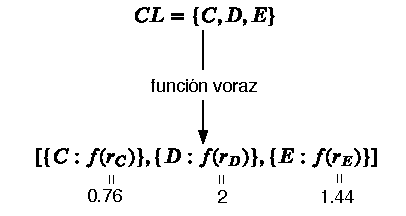
\includegraphics[scale=2]{Figures/proc-const/func-voraz.pdf}
	\caption{\footnotesize Ejemplo de obtención del listado de valores mediante la función voraz.}
	\label{fig:const:func-voraz}
\end{figure}

De este listado de valores se obtienen el valor máximo $\mathrm{g_{max}}=2$, y el mínimo $\mathrm{g_{min}}=0.76$. Con estos y el valor de $\alpha = 0.5$ por ejemplo, se calculará el valor de $\mu$ de la siguiente manera:
\begin{center}
	$\mu = 2 - 0.5 * (2 - 0.76) = 1.38$
\end{center}

Con este valor, se marca el umbral de selección para la lista restringida de candidatos o $RCL$, como se indica en la figura \ref{fig:const:rlc}, donde se incluirían solamente los nodos $D$ y $E$. De esta lista será seleccionado aleatoriamente un nodo, por ejemplo $D$, que será añadido a la solución parcial, quedando como $S = \{A, B, D\}$. Acto seguido, se eliminarán de $CL$ todos los nodos que no sean adyacentes a $D$ y se volverá a repetir este proceso descrito hasta que $CL$ quede vacía.

\begin{figure}[H]
	\centering
	\includegraphics[scale=2]{Figures/proc-const/rcl.pdf}
	\caption{\footnotesize Ejemplo de obtención de la lista de candidatos restringida.}
	\label{fig:const:rlc}
\end{figure}

%
%\begin{figure}[H]
%	\hspace{-1.5cm}
%	\begin{minipage}[b]{0.55\linewidth}
%		\centering
%		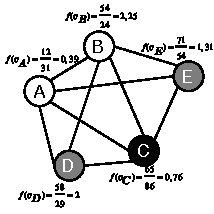
\includegraphics[scale=1.6]{Figures/diag-const-ratio.pdf}
%		\caption{\footnotesize Elección de nodo por mayor ratio.}
%		\label{fig:const-ratio}
%	\end{minipage}
%	\hspace{-1cm}
%	\begin{minipage}[b]{0.6\linewidth}
%		\centering
%		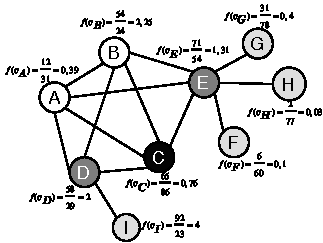
\includegraphics[scale=1.6]{Figures/diag-const-ady.pdf}
%		\caption{\footnotesize Elección de nodo por mayor número de adyacentes.}
%		\label{fig:const-ady}
%	\end{minipage}
%\end{figure}
%En el caso de la figura \ref{fig:const-ratio} se escoge el nodo $D$ que tiene una relación mayor entre sus pesos $p$ y $q$, $f(v_D)=\frac{58}{29}=2$, respecto del nodo $E$. Como siempre se selecciona un solo nodo en el paso \ref{alg:const_voraz:get_mejor} del algoritmo \ref{alg:const_voraz}, en lugar de un subconjunto de nodos, este caso puede suponer un mayor ratio final.
%
%Por otro lado, en la figura \ref{fig:const-ady}, se observa la opción de escoger el nodo con mayor número de vecinos. A priori, puede suponer una mejor solución añadir mayor cantidad de adyacentes y, por lo tanto, mayor ratio. Al tratarse de un algoritmo voraz, esta estrategia puede dejar atrás nodos más prometedores para alcanzar mayor ratio en la solución final. En este ejemplo, se escoge como mejor nodo el $E$, ya que tiene más adyacentes. Posteriormente se añade, por ejemplo, el nodo $G$, obteniendo un ratio de $f(\{v_A,v_B,v_C,v_E,v_G\})=0,96$. Esta selección está dejando atrás los nodos $D$ e $I$, los cuáles aportan mayor ratio a la solución, con un valor en este caso de $f(\{v_A,v_B,v_C,v_D,v_I\})=1,46$, superior al obtenido mediante el otro constructivo.

\subsection{Fase de mejora}
\label{sec:faseBusqueda}
Para esta segunda fase, se ha definido el algoritmo \ref{alg:bl}, el cuál parte de la solución obtenida previamente en la fase constructiva, formada por los nodos que forman un clique.

\begin{algorithm}
	$ soluciones \gets [] $ \\[0.2cm]
	$ vecinos \gets \emptyset $ \\[0.2cm] \label{alg:mj:vecVacios}
	$ vecinos \gets obtenerVecinos(solucion)$ \\[0.2cm] \label{alg:mj:getVecSol}
	$ vecinosOrdenados \gets ordenarVecinos(vecinos)$ \\[0.2cm] \label{alg:mj:ordVecs}
	\For{nodo $\epsilon$ vecinosOrdenados}{ \label{alg:mj:for}
		$ solucion\_parcial \gets incluirNodo(solucion, nodo) $ \\[0.2cm] \label{alg:mj:addNodoSol}
		\If{$ no \hspace{0.1cm} esClique(solucion) $}{ \label{alg:mj:conNoClique}
			$ solucion\_parcial \gets excluirNodos(solucion, nodo) $ \\[0.2cm] \label{alg:mj:exNodo}
		}\Else{
			$ solucion\_parcial \gets incluirAdyacentes(solucion\_parcial, nodo) $ \\[0.2cm] \label{alg:mj:addAdys}
			$ soluciones \gets incluirSolucion(solucion\_parcial) $
			 \\[0.2cm] \label{alg:mj:inclSolParc} 
		}
	}
	$ solucion \gets seleccionarMejorSolucion(soluciones) $
	\\[0.2cm] \label{alg:mj:selMejorSol}
	\Return solucion \label{alg:mj:rtSol}
	\caption{Pseudocódigo del algoritmo de búsqueda local.}
	\label{alg:bl}
\end{algorithm}

Con esta solución se obtienen en el paso \ref{alg:mj:getVecSol} todos los vecinos de cada nodo. Estos son ordenados de mayor a menor ratio en el paso \ref{alg:mj:ordVecs}.\\
Siguiendo con el ejemplo de la fase anterior nos quedaría un listado de nodos vecinos. Esta ordenación se realiza con el fin de aumentar las posibilidades de obtener un mejor valor de ratio. 

Se obtiene el primer nodo del listado y se añade a la solución en el paso \ref{alg:mj:addNodoSol}, comprobando posteriormente si esta solución forma o no un nuevo clique en el paso \ref{alg:mj:conNoClique}. Esta comprobación verifica que todos los nodos son adyacentes entre sí, formando un clique.

Si añadir el nodo no formara una solución, en el paso \ref{alg:mj:exNodo} se excluyen todos los nodos que impiden que se forme una solución factible.\\
En caso contrario, ese nodo añadido en el paso \ref{alg:mj:addNodoSol} se mantendría y a su vez, en el paso \ref{alg:mj:addAdys}, se añadirían todos sus nodos adyacentes, con el fin de obtener un clique de tamaño máximo, como marca la restricción del problema. El criterio de selección de los adyacentes es al igual que en la fase anterior, mediante una función voraz, en este caso por mayor ratio de entre los adyacentes disponibles.


Esa solución parcial es añadida al listado soluciones en el paso \ref{alg:mj:inclSolParc}. Tras procesarse todos los nodos, se seleccionará la solución con mayor ratio calculado y será retornada en el paso \ref{alg:mj:rtSol}.

A continuación, al igual que en la fase anterior se muestra un ejemplo del proceso.

Partiendo de una posible solución previa $ S=\{A, B, C, D, E\} $, en la figura \ref{fig:bl:adys} se muestra la lista ordenada por ratio de todos los nodos adyacentes de la solución previa. 

\begin{figure}[H]
	\centering
	
\includegraphics[scale=2]{Figures/proc-bl/adys-ord.pdf}
	\caption{\footnotesize Lista de adyacentes ordenada.}
	\label{fig:bl:adys}
\end{figure}

De este listado se selecciona la primera posición correspondiente en este caso con el nodo $A_1$ ya que tiene el mayor ratio y es añadido a la solución parcial $S_{A_1}$.

A continuación se comprueba si esta nueva solución cumple con las restricciones para ser clique. Si no cumple con las restricciones se aplicaría el proceso de exclusión de nodos que evitan que se forme un clique. En la imagen \ref{fig:bl:exc} se muestra el proceso, en el que los nodos sombreados $B$ y $C$ son eliminados de la solución.

\begin{figure}[H]
	\centering
	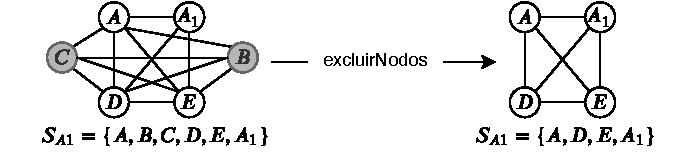
\includegraphics[scale=1.3]{Figures/proc-bl/excluirNodos.pdf}
	\caption{\footnotesize Exclusión de los nodos que impiden obtener un clique factible.}
	\label{fig:bl:exc}
\end{figure}

Una vez se tiene una solución parcial factible, se añaden todos los nodos adyacentes a los de la solución para obtener un clique máximo. En la figura \ref{fig:bl:add-ayd} se muestra el proceso de adición de los adyacentes mediante una función voraz, en este caso el criterio de selección es por el que aporte mayor ratio a esa solución parcial. Como se indicó anteriormente este ratio es calculado con los pesos $p$ y $q$ asociados al nodo en cuestión.

 Esta será añadida al listado de soluciones parciales.

\begin{figure}[H]
	\centering
	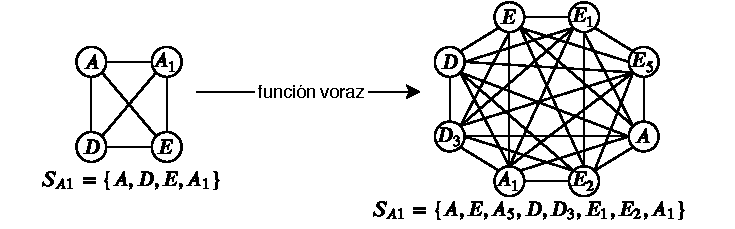
\includegraphics[scale=1.3]{Figures/proc-bl/add-adys.pdf}
	\caption{\footnotesize Adición de adyacentes a la solución parcial.}
	\label{fig:bl:add-ayd}
\end{figure}

Este proceso será repetido con todos los nodos de la lista ordenada generada al inicio y finalmente se devolverá la solución que ha obtenido mayor valor de ratio calculado.

%-------------------------------------------------------------------------------